\begin{frame}
\frametitle{$DC_C$ Calculus: Structure}
%make tikz pic?
%three components: Constraint System, Op Semantics, Type Rel
%arrows from constraints sys to op sem and type rel
%with label Uses/Used in
\centering
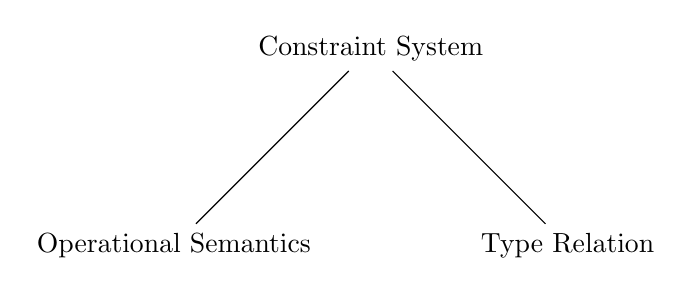
\begin{tikzpicture}
  \node (cs) at (0,1) {Constraint System};
  \node (sem) at (-2.5,-1.5) {Operational Semantics};
  \node (type) at (2.5,-1.5) {Type Relation};
  \path (cs) edge (sem);
  \path (cs) edge (type);
% \node (comment) at (-0.5, -0.5) {asdf};
\end{tikzpicture}
\end{frame}

\begin{frame}
\frametitle{$DC_C$ Calculus: General Syntax}

\begin{align*}
p, q \in \mathit{Path} &::= x \ |\ \mathit{p.f}\\
a, b, c \in \mathit{Constr} &::= \pathEq{p}{q}\\
                &\ \ |\ \instOf{p}{C}\\
                &\ \ |\ \instBy{p}{C}\\
t \in \mathit{Type} &::= \type{x}{\ovl{a}}
\end{align*}
%$x$ - variable names
%$f$ - field names
%$C$ - class names
%$m$ - method names
\end{frame}

\begin{frame}
\frametitle{$DC_C$ Calculus: Expressions \& Programs}

\begin{columns}[t]
\begin{column}{0.4\linewidth}
\begin{align*}
\quad\\
e \in \mathit{Expr} &::= x\\
              &\ \ |\ \mathit{e.f}\\
              &\ \ |\ \newInst{C}{\overline{f}}{\overline{e}}\\
              &\ \ |\ m(\mathit{e})
\end{align*}
\end{column}
\begin{column}{0.58\linewidth}
\begin{align*}
P \in \mathit{Program} &::= \ovl{D} \\
D \in \mathit{Decl} &::= \constr{C}{x}{\overline{a}}\\
              &\ \ |\ \progEnt{x}{\overline{a}}{a}\\
              &\ \ |\ \mDecl{m}{x}{\overline{a}}{t}\\
              &\ \ |\ \mImpl{m}{x}{\overline{a}}{t}{e}
\end{align*}
\end{column}
\end{columns}
\end{frame}

\begin{frame}
\frametitle{$DC_C$ Calculus: Natural Numbers Program}

\begin{align*}
&\constr{\texttt{Zero}}{x}{\epsilon}\\
&\progEnt{x}{\instOf{x}{\texttt{Zero}}}{\instOf{x}{\texttt{Nat}}}\\
&\constr{\texttt{Succ}}{x}{\instOf{x.p}{\texttt{Nat}}}\\
&\progEnt{x}{\instOf{x}{\texttt{Succ}}, \instOf{x.p}{\texttt{Nat}}}{\instOf{x}{\texttt{Nat}}}\\
&\mDecl{\texttt{prev}}{x}{\instOf{x}{\texttt{Nat}}}{\type{y}{\instOf{y}{\texttt{Nat}}}}\\
&\mImpl{\texttt{prev}}{x}{\instOf{x}{\texttt{Zero}}}{\type{y}{\instOf{y}{\texttt{Nat}}}}{\newInstNoArgs{\texttt{Zero}}}\\
&\mImpl{\texttt{prev}}{x}{\instOf{x}{\texttt{Succ}}, \instOf{x.p}{\texttt{Nat}}}{\type{y}{\instOf{y}{\texttt{Nat}}}}{x.p}
\end{align*}
\end{frame}
